% Options for packages loaded elsewhere
\PassOptionsToPackage{unicode}{hyperref}
\PassOptionsToPackage{hyphens}{url}
%
\documentclass[
  12pt,
  ignorenonframetext,
  aspectratio=169,
]{beamer}
\usepackage{pgfpages}
\setbeamertemplate{caption}[numbered]
\setbeamertemplate{caption label separator}{: }
\setbeamercolor{caption name}{fg=normal text.fg}
\beamertemplatenavigationsymbolsempty
% Prevent slide breaks in the middle of a paragraph
\widowpenalties 1 10000
\raggedbottom
\setbeamertemplate{part page}{
  \centering
  \begin{beamercolorbox}[sep=16pt,center]{part title}
    \usebeamerfont{part title}\insertpart\par
  \end{beamercolorbox}
}
\setbeamertemplate{section page}{
  \centering
  \begin{beamercolorbox}[sep=12pt,center]{part title}
    \usebeamerfont{section title}\insertsection\par
  \end{beamercolorbox}
}
\setbeamertemplate{subsection page}{
  \centering
  \begin{beamercolorbox}[sep=8pt,center]{part title}
    \usebeamerfont{subsection title}\insertsubsection\par
  \end{beamercolorbox}
}
\AtBeginPart{
  \frame{\partpage}
}
\AtBeginSection{
  \ifbibliography
  \else
    \frame{\sectionpage}
  \fi
}
\AtBeginSubsection{
  \frame{\subsectionpage}
}

\usepackage{amsmath,amssymb}
\usepackage{iftex}
\ifPDFTeX
  \usepackage[T1]{fontenc}
  \usepackage[utf8]{inputenc}
  \usepackage{textcomp} % provide euro and other symbols
\else % if luatex or xetex
  \usepackage{unicode-math}
  \defaultfontfeatures{Scale=MatchLowercase}
  \defaultfontfeatures[\rmfamily]{Ligatures=TeX,Scale=1}
\fi
\usepackage{lmodern}
\usetheme[]{Rochester}
\usecolortheme{spruce}
\usefonttheme{professionalfonts}
\ifPDFTeX\else  
    % xetex/luatex font selection
\fi
% Use upquote if available, for straight quotes in verbatim environments
\IfFileExists{upquote.sty}{\usepackage{upquote}}{}
\IfFileExists{microtype.sty}{% use microtype if available
  \usepackage[]{microtype}
  \UseMicrotypeSet[protrusion]{basicmath} % disable protrusion for tt fonts
}{}
\makeatletter
\@ifundefined{KOMAClassName}{% if non-KOMA class
  \IfFileExists{parskip.sty}{%
    \usepackage{parskip}
  }{% else
    \setlength{\parindent}{0pt}
    \setlength{\parskip}{6pt plus 2pt minus 1pt}}
}{% if KOMA class
  \KOMAoptions{parskip=half}}
\makeatother
\usepackage{xcolor}
\newif\ifbibliography
\setlength{\emergencystretch}{3em} % prevent overfull lines
\setcounter{secnumdepth}{-\maxdimen} % remove section numbering


\providecommand{\tightlist}{%
  \setlength{\itemsep}{0pt}\setlength{\parskip}{0pt}}\usepackage{longtable,booktabs,array}
\usepackage{calc} % for calculating minipage widths
\usepackage{caption}
% Make caption package work with longtable
\makeatletter
\def\fnum@table{\tablename~\thetable}
\makeatother
\usepackage{graphicx}
\makeatletter
\def\maxwidth{\ifdim\Gin@nat@width>\linewidth\linewidth\else\Gin@nat@width\fi}
\def\maxheight{\ifdim\Gin@nat@height>\textheight\textheight\else\Gin@nat@height\fi}
\makeatother
% Scale images if necessary, so that they will not overflow the page
% margins by default, and it is still possible to overwrite the defaults
% using explicit options in \includegraphics[width, height, ...]{}
\setkeys{Gin}{width=\maxwidth,height=\maxheight,keepaspectratio}
% Set default figure placement to htbp
\makeatletter
\def\fps@figure{htbp}
\makeatother

\usepackage{booktabs}
\usepackage{longtable}
\usepackage{array}
\usepackage{multirow}
\usepackage{wrapfig}
\usepackage{float}
\usepackage{colortbl}
\usepackage{pdflscape}
\usepackage{tabu}
\usepackage{threeparttable}
\usepackage{threeparttablex}
\usepackage[normalem]{ulem}
\usepackage{makecell}
\usepackage{xcolor}
\usepackage{graphicx}
\usepackage{svg}
\makeatletter
\makeatother
\makeatletter
\makeatother
\makeatletter
\@ifpackageloaded{caption}{}{\usepackage{caption}}
\AtBeginDocument{%
\ifdefined\contentsname
  \renewcommand*\contentsname{Table of contents}
\else
  \newcommand\contentsname{Table of contents}
\fi
\ifdefined\listfigurename
  \renewcommand*\listfigurename{List of Figures}
\else
  \newcommand\listfigurename{List of Figures}
\fi
\ifdefined\listtablename
  \renewcommand*\listtablename{List of Tables}
\else
  \newcommand\listtablename{List of Tables}
\fi
\ifdefined\figurename
  \renewcommand*\figurename{Figure}
\else
  \newcommand\figurename{Figure}
\fi
\ifdefined\tablename
  \renewcommand*\tablename{Table}
\else
  \newcommand\tablename{Table}
\fi
}
\@ifpackageloaded{float}{}{\usepackage{float}}
\floatstyle{ruled}
\@ifundefined{c@chapter}{\newfloat{codelisting}{h}{lop}}{\newfloat{codelisting}{h}{lop}[chapter]}
\floatname{codelisting}{Listing}
\newcommand*\listoflistings{\listof{codelisting}{List of Listings}}
\makeatother
\makeatletter
\@ifpackageloaded{caption}{}{\usepackage{caption}}
\@ifpackageloaded{subcaption}{}{\usepackage{subcaption}}
\makeatother
\makeatletter
\@ifpackageloaded{tcolorbox}{}{\usepackage[skins,breakable]{tcolorbox}}
\makeatother
\makeatletter
\@ifundefined{shadecolor}{\definecolor{shadecolor}{rgb}{.97, .97, .97}}
\makeatother
\makeatletter
\makeatother
\makeatletter
\makeatother
\ifLuaTeX
  \usepackage{selnolig}  % disable illegal ligatures
\fi
\IfFileExists{bookmark.sty}{\usepackage{bookmark}}{\usepackage{hyperref}}
\IfFileExists{xurl.sty}{\usepackage{xurl}}{} % add URL line breaks if available
\urlstyle{same} % disable monospaced font for URLs
\hypersetup{
  pdftitle={ERA 5 calibration to Elexon power},
  pdfauthor={S. Gomez\^{}1},
  hidelinks,
  pdfcreator={LaTeX via pandoc}}

\title{ERA 5 calibration to Elexon power}
\author{S. Gomez\(^1\)}
\date{2025-11-04}
\institute{\(^1\)School of Mathematics, University of Edinburgh}

\begin{document}
\frame{\titlepage}
\ifdefined\Shaded\renewenvironment{Shaded}{\begin{tcolorbox}[frame hidden, borderline west={3pt}{0pt}{shadecolor}, interior hidden, enhanced, sharp corners, boxrule=0pt, breakable]}{\end{tcolorbox}}\fi

\renewcommand*\contentsname{Table of contents}
\begin{frame}[allowframebreaks]
  \frametitle{Table of contents}
  \tableofcontents[hideallsubsections]
\end{frame}
\hypertarget{sec-intro}{%
\section{Calibration to power}\label{sec-intro}}

\begin{frame}{Updates}
\protect\hypertarget{updates}{}
\begin{itemize}
\tightlist
\item
  Curtailment data to obtain potential generation
\item
  Outage data to exclude periods where capacity is constrained
\item
  Power curve comparison to data
\item
  ERA 5 wind speed conversion to power
\end{itemize}
\end{frame}

\begin{frame}{ERA5 vs Elexon generation}
\protect\hypertarget{era5-vs-elexon-generation}{}
Calibrate a ERA5 driven estimate to actual observed output accounting
for spatiotemporal properties.

\vspace{0.2cm}
\begin{columns}[T, totalwidth=\textwidth]
  \begin{column}{0.5\textwidth}
    \centering
    \textbf{\small ERA5 at wind farms}\\[0.5em]
    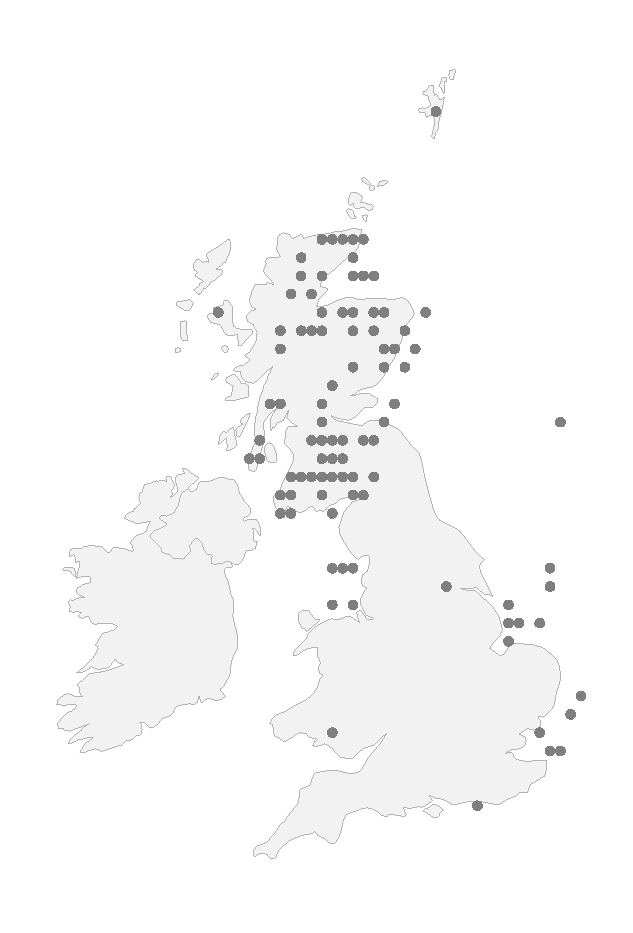
\includegraphics[width=\linewidth,height=5cm,keepaspectratio]{../fig/era5_at_windfarms.eps}
  \end{column}

  \begin{column}{0.5\textwidth}
    \centering
    \textbf{\small Elexon wind farms map (2025)}\\[0.5em]
    \vspace{-0.2cm}
    \includegraphics[width=\linewidth,height=5cm,keepaspectratio]{../fig/wind_farms_elexon_size_2025.jpeg}
  \end{column}
\end{columns}
\end{frame}

\hypertarget{sec-gwa}{%
\section{ERA5}\label{sec-gwa}}

\begin{frame}{Characteristics}
\protect\hypertarget{characteristics}{}
\begin{columns}[T, totalwidth=\textwidth]
   \begin{column}{0.4\textwidth}
    % set font size for itemize levels locally
    {
    \setbeamerfont{itemize/enumerate body}{size=\fontsize{9}{10}\selectfont}
    \setbeamerfont{itemize/enumerate subbody}{size=\fontsize{8}{10}\selectfont}

    \begin{itemize}
      \item 5th generation of ECMWF's global reanalysis
      \item Spatial resolution $0.25^\circ \times 0.25^\circ$ (31km $\times$ 31 km at equator)
      \item Hourly temporal resolution
      \item Heights: 10m, 100m
    \end{itemize}
    } % end local font block
  \end{column}

  % Right column: figure
  
  \begin{column}{0.6\textwidth}
    \centering
    \small Average monthly wind speed and 90 CI
    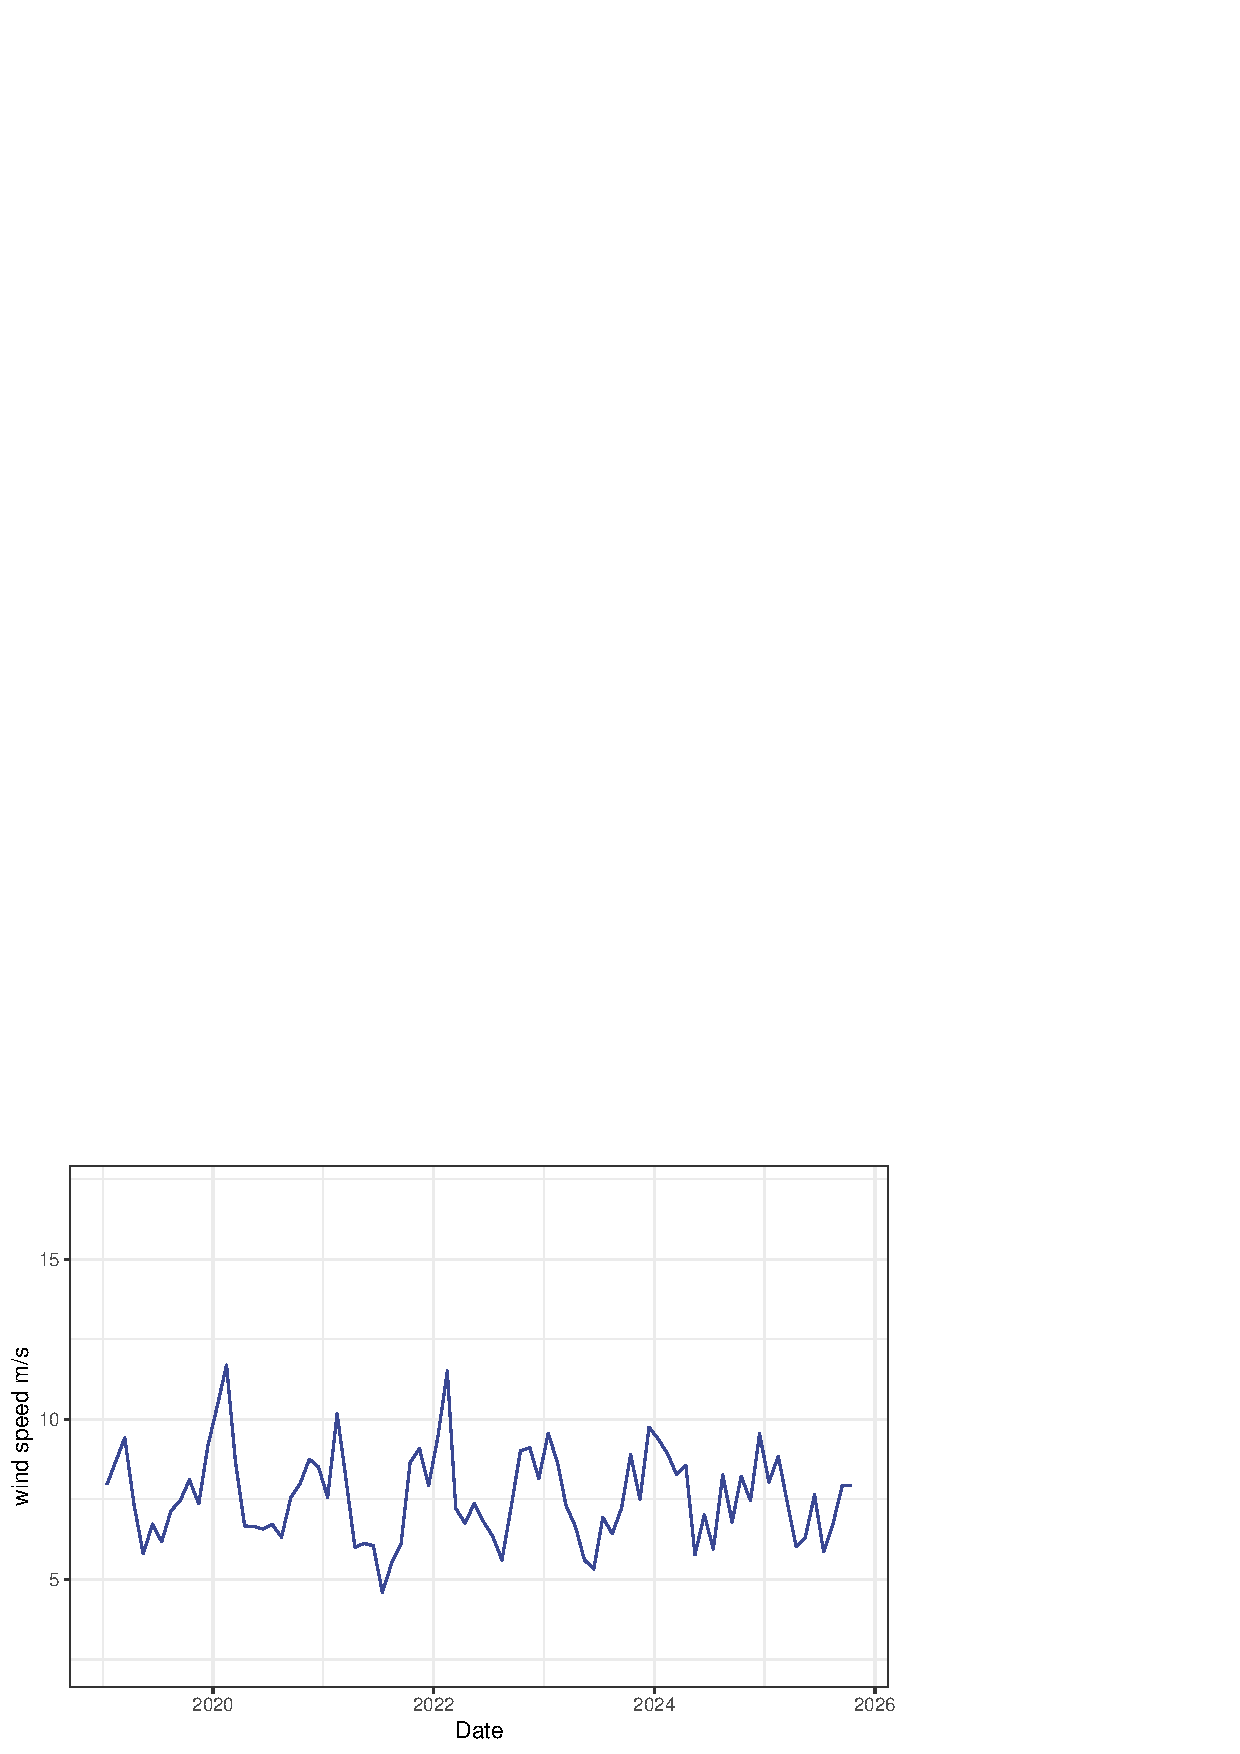
\includegraphics[width=\linewidth,height=5cm,keepaspectratio]{../fig/ws_uk_1s.pdf}
  \end{column}

\end{columns}
\end{frame}

\begin{frame}{ERA5 series}
\protect\hypertarget{era5-series}{}
\begin{columns}[T]
\begin{column}{0.5\textwidth}
\centering

\small Wind speed seasonality
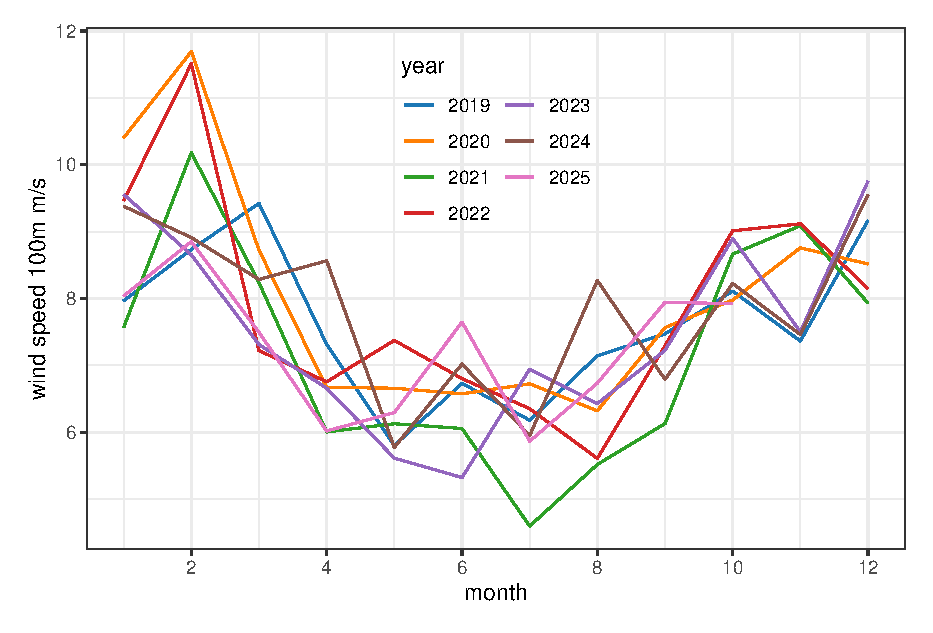
\includegraphics[width=\linewidth,height=5cm,keepaspectratio]{../fig/ws_uk_1s_seas.eps}
\end{column}

\begin{column}{0.5\textwidth}
\centering

\small Wind speed by location type
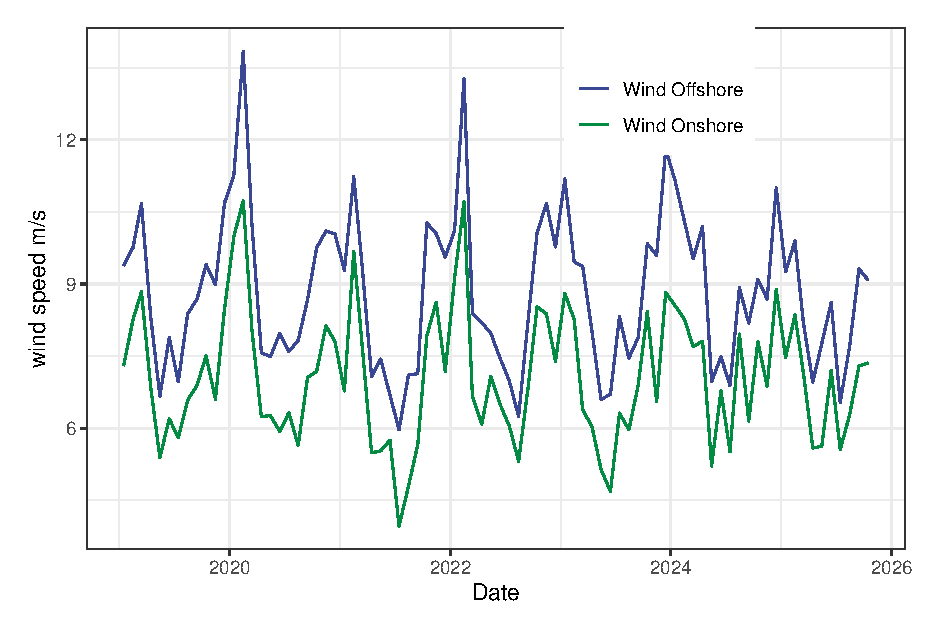
\includegraphics[width=\linewidth,height=5cm,keepaspectratio]{../fig/ws_uk_tech.eps}
\end{column}
\end{columns}
\end{frame}

\begin{frame}{ERA5 wind direction at wind farms}
\protect\hypertarget{era5-wind-direction-at-wind-farms}{}
\begin{columns}[T]
\begin{column}{0.5\textwidth}
\centering

\small Wind direction frequency
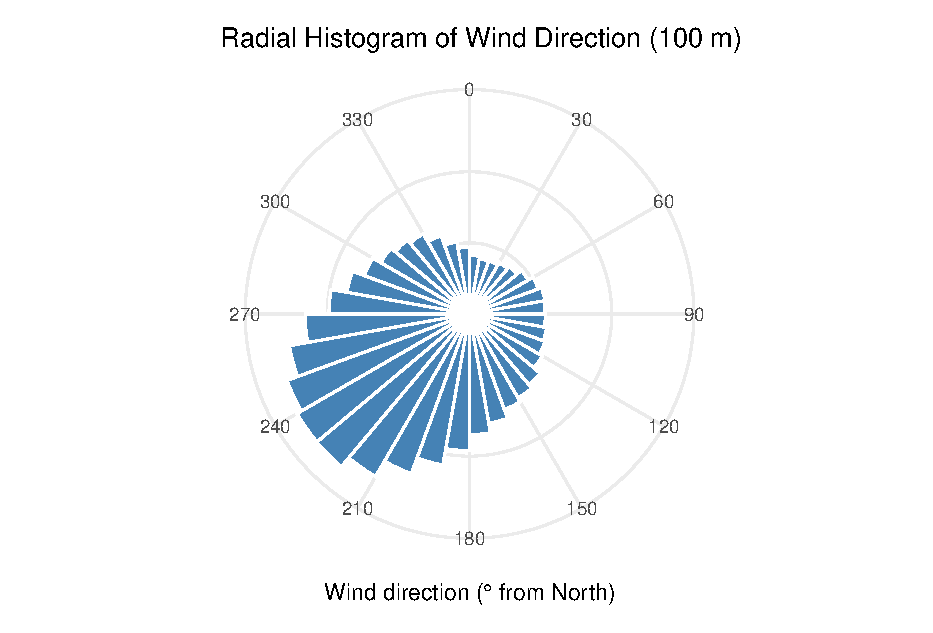
\includegraphics[width=\linewidth,height=5cm,keepaspectratio]{../fig/wd_uk_1s.eps}
\end{column}

\begin{column}{0.7\textwidth}
\centering

\small Seasonal patterns
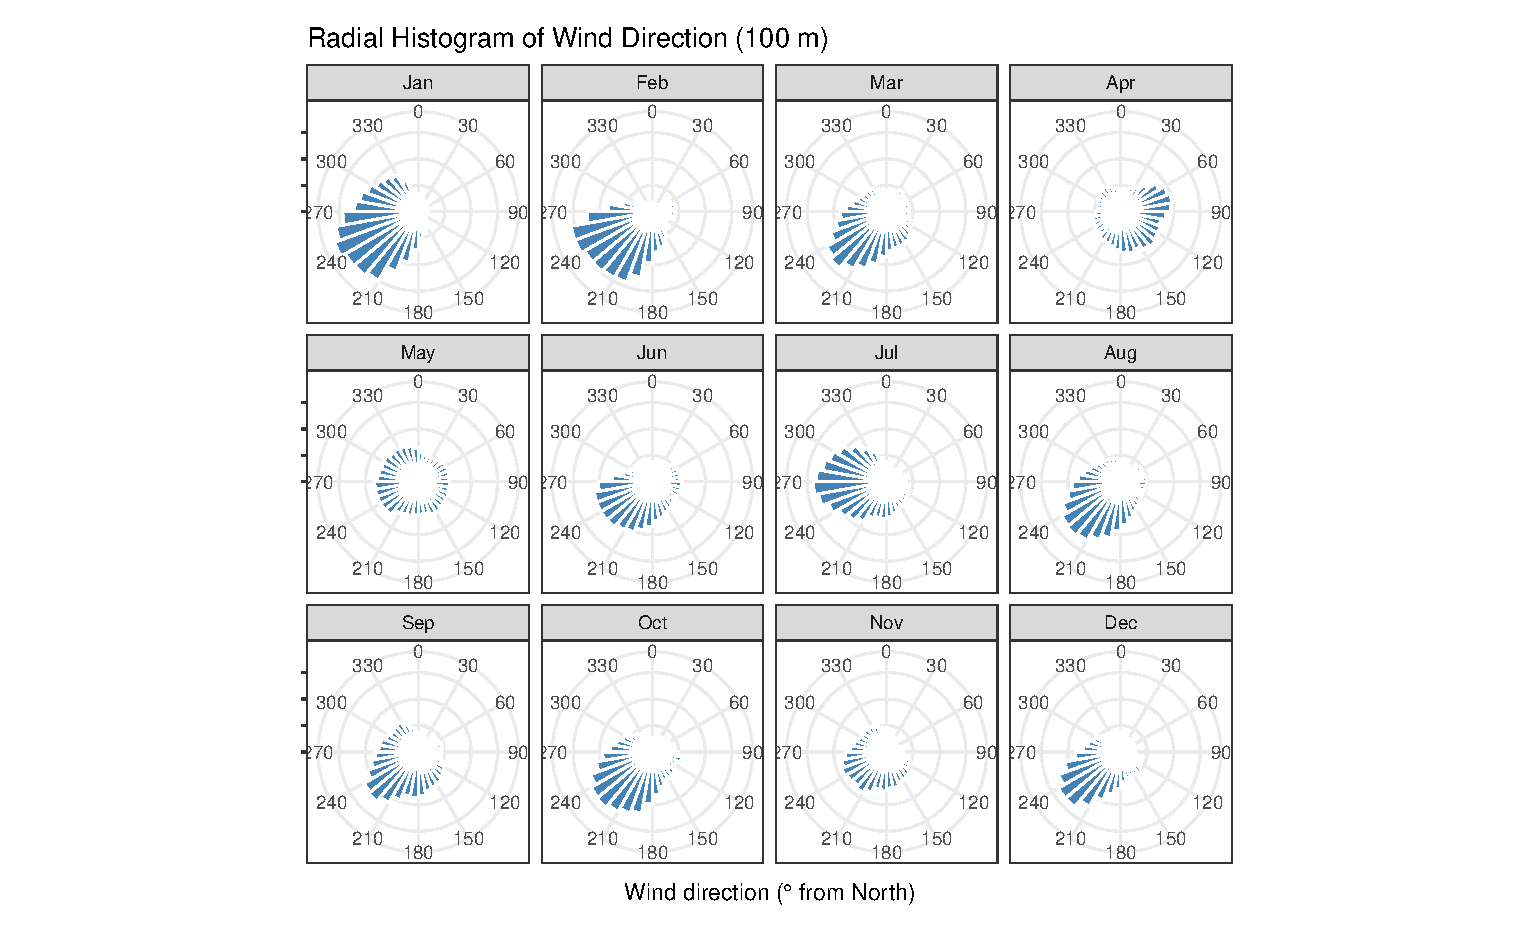
\includegraphics[width=\linewidth,height=7cm,keepaspectratio]{../fig/wd_uk_1s_seas.eps}
\end{column}
\end{columns}
\end{frame}

\hypertarget{sec-elexon}{%
\section{Elexon data}\label{sec-elexon}}

\begin{frame}{BMU wind data}
\protect\hypertarget{bmu-wind-data}{}
\begin{columns}[T, totalwidth=\textwidth]
   \begin{column}{0.5\textwidth}
    % set font size for itemize levels locally
    {
    \setbeamerfont{itemize/enumerate body}{size=\fontsize{9}{10}\selectfont}
    \setbeamerfont{itemize/enumerate subbody}{size=\fontsize{8}{10}\selectfont}

    \begin{itemize}
      \item 150 wind farms split in over 216 units
      \item Total capacity: 27 GW
      \item Half hourly resolution
      \item Records starting in 2019
      \item Curtailment and outage data available
      \item Location / turbine data unavailable
    \end{itemize}
    } % end local font block
  \end{column}

  % Right column: figure
  \begin{column}{0.5\textwidth}
    \centering
    \small Wind installed capacity
    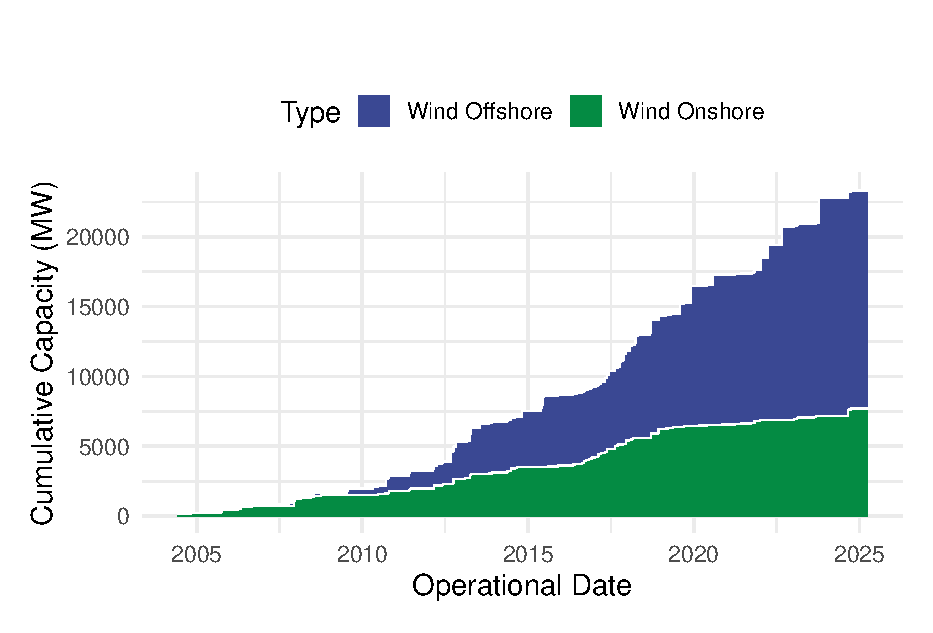
\includegraphics[width=\linewidth,height=5cm,keepaspectratio]{../fig/wind_capacity_type_2025_nt.eps}
  \end{column}

\end{columns}
\end{frame}

\begin{frame}{BMU wind data}
\protect\hypertarget{bmu-wind-data-1}{}
\small BMU wind generation (2024)

\begin{table}
\centering
\resizebox{\ifdim\width>\linewidth\linewidth\else\width\fi}{!}{
\begin{tabular}{l|r|r|r|r|r|r|r}
\hline
Type & Generation (GWh) & Curtailment & Potential & Capacity (MW) & Number of BMUs & CF & PF\\
\hline
Wind Offshore & 46,907 & 4,902 & 51,810 & 15,563 & 80 & 0.42 & 0.47\\
\hline
Wind Onshore & 16,254 & 3,363 & 19,617 & 7,860 & 123 & 0.29 & 0.34\\
\hline
Total & 63,162 & 8,266 & 71,427 & 23,423 & 203 & 0.37 & 0.42\\
\hline
\end{tabular}}
\end{table}
\end{frame}

\begin{frame}{Capacity factor through time}
\protect\hypertarget{capacity-factor-through-time}{}
\begin{columns}[T]
\begin{column}{0.5\textwidth}
\centering

\small Capacity factor by year
\includegraphics[width=\linewidth,height=5cm,keepaspectratio]{../fig/capacity_factor2.pdf}
\end{column}

\begin{column}{0.5\textwidth}
\centering

\small Capacity factor by quarter
\includegraphics[width=\linewidth,height=5cm,keepaspectratio]{../fig/capacity_factor2_q.pdf}
\end{column}
\end{columns}
\end{frame}

\begin{frame}{Curtailment through time}
\protect\hypertarget{curtailment-through-time}{}
\begin{columns}[T]
\begin{column}{0.5\textwidth}
\centering

\small Curtailment by year
\includegraphics[width=\linewidth,height=5cm,keepaspectratio]{../fig/curtailment_factor.pdf}
\end{column}

\begin{column}{0.5\textwidth}
\centering

\small Curtailment seasonality
\includegraphics[width=\linewidth,height=5cm,keepaspectratio]{../fig/curtailment_factor_q.pdf}
\end{column}
\end{columns}
\end{frame}

\begin{frame}{Potential generation}
\protect\hypertarget{potential-generation}{}
\begin{columns}[T]
\begin{column}{0.5\textwidth}
\centering

\small Potential by year
\includegraphics[width=\linewidth,height=5cm,keepaspectratio]{../fig/potential_factor.pdf}
\end{column}

\begin{column}{0.5\textwidth}
\centering

\small Potential seasonality
\includegraphics[width=\linewidth,height=5cm,keepaspectratio]{../fig/potential_factor_q.pdf}
\end{column}
\end{columns}
\end{frame}

\begin{frame}{Renewable energy planning database (REPD)}
\protect\hypertarget{renewable-energy-planning-database-repd}{}
\begin{columns}[T]
\begin{column}{0.5\textwidth}
\setbeamerfont{itemize/enumerate body}{size=\fontsize{9}{10}\selectfont}
\setbeamerfont{itemize/enumerate subbody}{size=\fontsize{8}{10}\selectfont}
\begin{itemize}
      \item Official UK government renewable data
      \item Over 800 wind farms listed as operational
      \item Coordinates available 
      \item Also available:
      \begin{itemize}
        \item Development status 
        \item Number of turbines
        \item Turbine capacity
        \item Turbine height (for some only)
      \end{itemize}
    \end{itemize}
\end{column}

\begin{column}{0.5\textwidth}
\centering

\small REPD wind farms \vspace{0.2cm}

\begin{table}
\centering
\resizebox{\ifdim\width>\linewidth\linewidth\else\width\fi}{!}{
\begin{tabular}{l|l|r|r}
\hline
Type & Development Status & Count & Capacity MW\\
\hline
Wind Offshore & Operational & 47 & 14,679\\
\hline
Wind Offshore & Under Construction & 7 & 7,742\\
\hline
Wind Onshore & Operational & 770 & 14,738\\
\hline
Wind Onshore & Under Construction & 37 & 1,779\\
\hline
Total & - & 861 & 38,938\\
\hline
\end{tabular}}
\end{table}
\end{column}
\end{columns}
\end{frame}

\begin{frame}{Turbine data available}
\protect\hypertarget{turbine-data-available}{}
\begin{columns}[T]
\begin{column}{0.5\textwidth}
\centering

\small Turbine capacity histogram
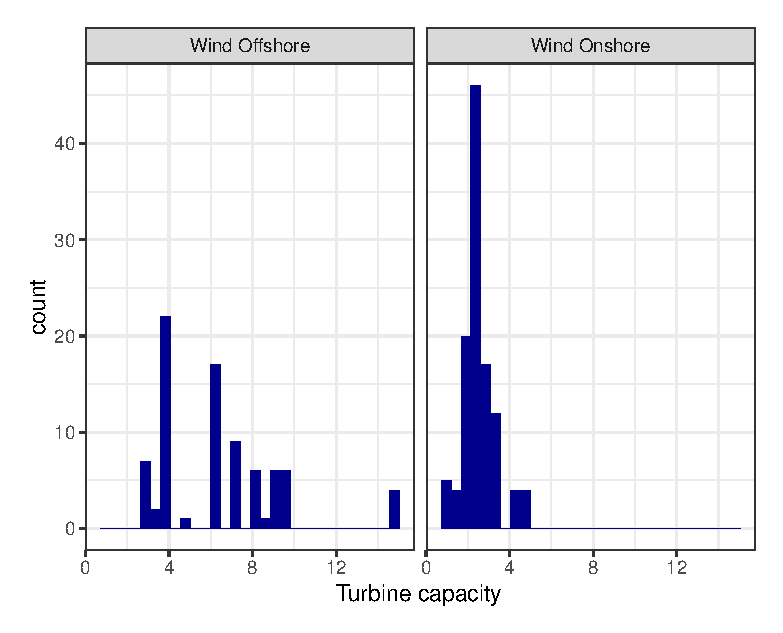
\includegraphics[width=\linewidth,height=5cm,keepaspectratio]{../fig/hist_turb_capacity_2025.eps}
\end{column}

\begin{column}{0.5\textwidth}
\centering

\small Number of turbines histogram
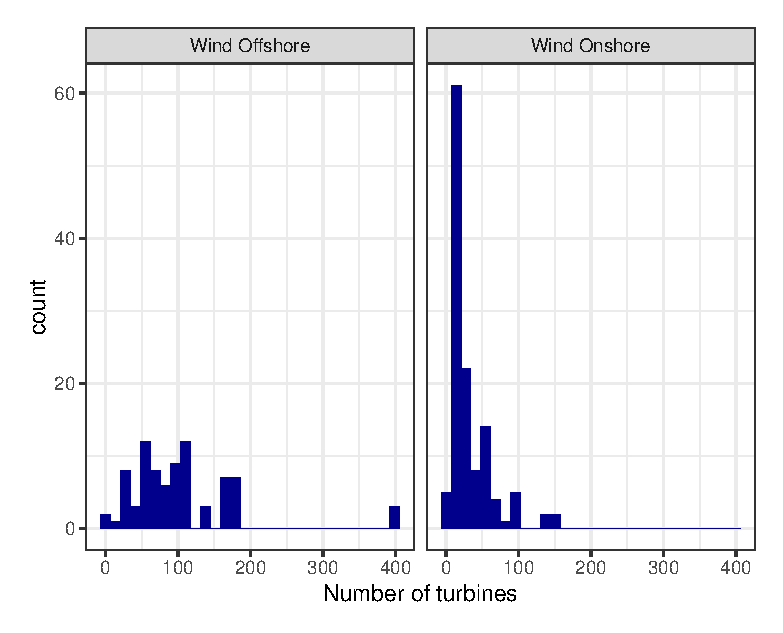
\includegraphics[width=\linewidth,height=5cm,keepaspectratio]{../fig/hist_n_turb_2025.eps}
\end{column}
\end{columns}
\end{frame}

\begin{frame}{Turbine data available}
\protect\hypertarget{turbine-data-available-1}{}
\begin{columns}[T]
\begin{column}{0.5\textwidth}
\centering

Turbine Height availability \vspace{1cm}

\begin{table}
\centering
\resizebox{\ifdim\width>\linewidth\linewidth\else\width\fi}{!}{
\begin{tabular}{l|l|r|r}
\hline
Type & Height available & Average height (m) & count\\
\hline
Wind Offshore & FALSE & 222.0 & 23\\
\hline
Wind Offshore & TRUE & NaN & 64\\
\hline
Wind Onshore & FALSE & 137.7 & 45\\
\hline
Wind Onshore & TRUE & NaN & 84\\
\hline
\end{tabular}}
\end{table}
\end{column}

\begin{column}{0.5\textwidth}
\centering

\small Turbine height histogram
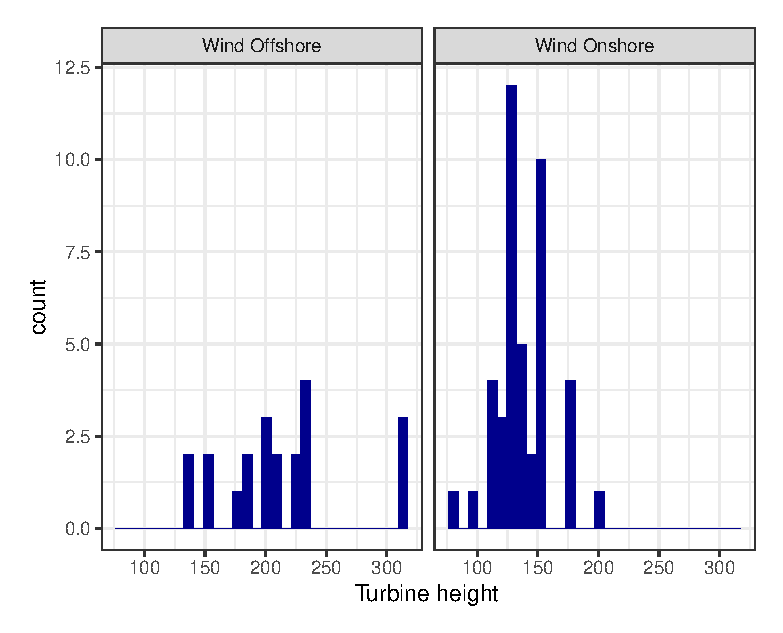
\includegraphics[width=\linewidth,height=5cm,keepaspectratio]{../fig/hist_turb_height_2025.eps}
\end{column}
\end{columns}
\end{frame}

\hypertarget{sec-power_curves}{%
\section{Power conversion}\label{sec-power_curves}}

\begin{frame}{Generic power curves}
\protect\hypertarget{generic-power-curves}{}
\begin{columns}[T]
\begin{column}{0.5\textwidth}
\setbeamerfont{itemize/enumerate body}{size=\fontsize{9}{10}\selectfont}
\setbeamerfont{itemize/enumerate subbody}{size=\fontsize{8}{10}\selectfont}
\begin{itemize}
      \item Using 3 generic power curves
      \item Offshore plus the IEC 3 classes
      \item Assigning class based on GWA mean wind speed at location
      \item Rescaling rated power to turbine capacity
\end{itemize}

\vspace{0.2cm}
\centering

IEC classification

\vspace{0.2cm}
\resizebox{\linewidth}{!}{%
\begin{tabular}{l c c l}
\toprule
Class & Mean wind speed  & Extreme 10-min & Typical sites \\
 & at hub height (m/s) &  gust (m/s) \\
\midrule
I   & 10   & 70   & Very windy / exposed sites \\
II  & 8.5  & 59.5 & Moderate wind sites \\
III & 7.5  & 52.5 & Low-wind / inland sites \\
\bottomrule
\end{tabular}
}
\end{column}

\begin{column}{0.5\textwidth}
\centering

\small Generic power curves (PC\(_k\))
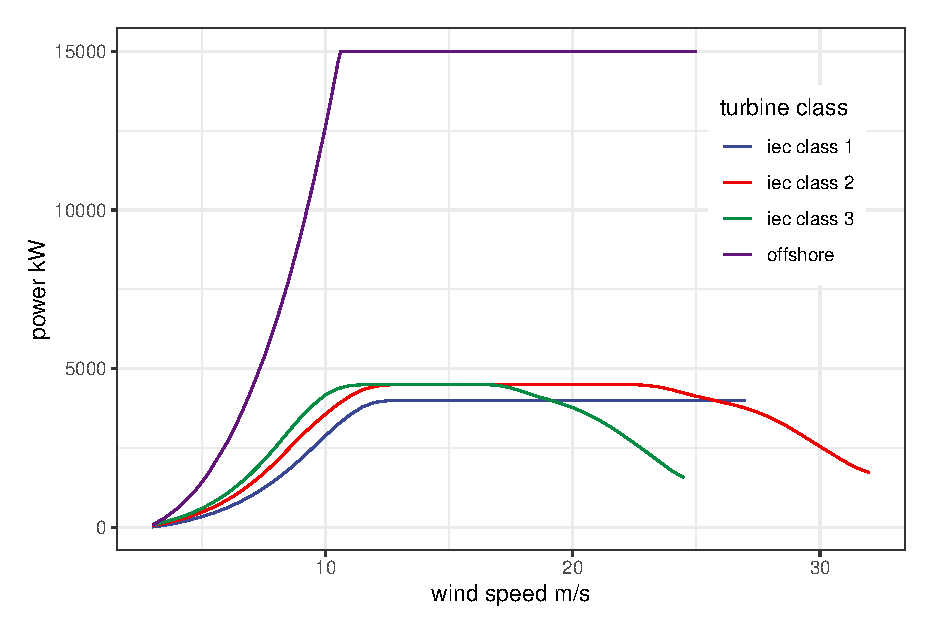
\includegraphics[width=\linewidth,height=5cm,keepaspectratio]{../fig/generic_power_curves_uncens.eps}
\end{column}
\end{columns}
\end{frame}

\begin{frame}{Power estimate based on generic power curves}
\protect\hypertarget{power-estimate-based-on-generic-power-curves}{}
For each location \(i\) we have:

\begin{itemize}
\tightlist
\item
  observed raw power \(\tilde p_{it}\)
\item
  curtailment amount \(a_{it}\)
\item
  potential output \(p_{it} = \tilde p_{it} + a_{it}\)
\item
  wind farm capacity \(c_i\)
\item
  turbine height \(v_i\)
\item
  ERA5 wind speed \(w_{it}\).
\end{itemize}
\end{frame}

\begin{frame}{Power estimate based on generic power curves}
\protect\hypertarget{power-estimate-based-on-generic-power-curves-1}{}
An initial estimate will require:

\begin{itemize}
  \item Mapping location to a rescaled power curve $\widetilde \text{PC}_k$
  \item Estimate wind farm power in GWh
\end{itemize}

\begin{equation*}
    \hat p_{it} = \widetilde \text{PC}_{k} (w_{it})
\end{equation*}
\end{frame}

\begin{frame}{Generic power curves vs observed data - Fallago Rig}
\protect\hypertarget{generic-power-curves-vs-observed-data---fallago-rig}{}
Onshore wind farm with moderate curtailment

\begin{columns}[T, totalwidth=\textwidth]

  \begin{column}{0.5\textwidth}
    \centering
    {\small Comparison with raw generation}
    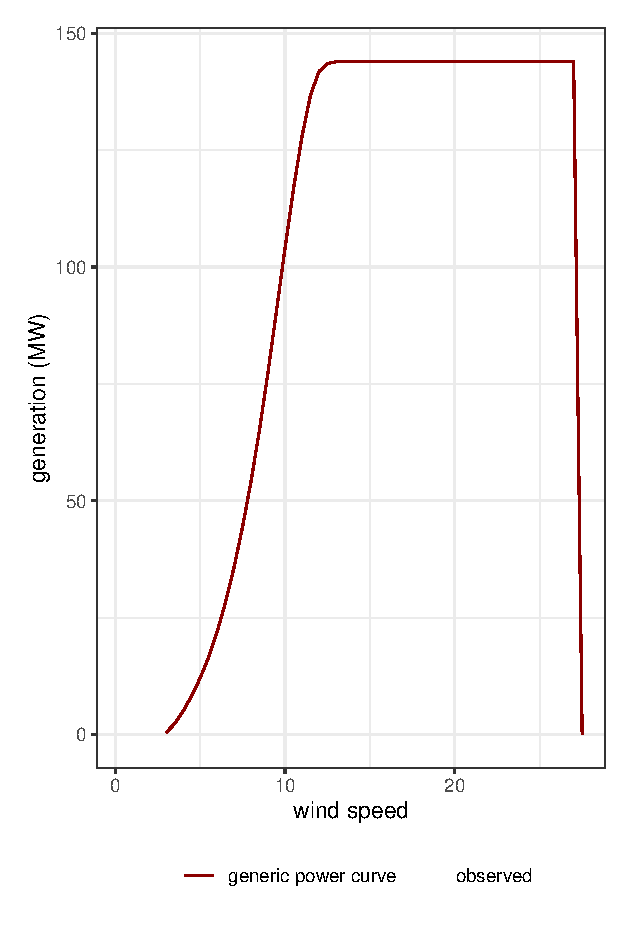
\includegraphics[
      width=\linewidth,
      height=5cm,keepaspectratio]{
        ../fig/pc_comparison_T_FALGW-1_valq0.pdf}
    
  \end{column}

  \begin{column}{0.5\textwidth}
    \centering
    {\small Adding curtailment}

    \includegraphics[
      width=\linewidth,
      height=5cm,keepaspectratio]{
        ../fig/pc_comparison_T_FALGW-1_valpot.pdf}
  \end{column}

\end{columns}
\end{frame}

\begin{frame}{Generic power curves vs observed data - Fallago Rig}
\protect\hypertarget{generic-power-curves-vs-observed-data---fallago-rig-1}{}
Onshore wind farm with moderate curtailment

\begin{columns}[T, totalwidth=\textwidth]

  \begin{column}{0.5\textwidth}
    \centering
    {\small Highlighting outages}
    \includegraphics[
      width=\linewidth,
      height=5cm,keepaspectratio]{
        ../fig/pc_comparison_T_FALGW-1_valout.pdf}
    
  \end{column}

  \begin{column}{0.5\textwidth}
    \centering
    {\small Potential generation excluding outages}

    \includegraphics[
      width=\linewidth,
      height=5cm,keepaspectratio]{
        ../fig/pc_comparison_T_FALGW-1_valnout.pdf}
  \end{column}

\end{columns}
\end{frame}

\begin{frame}{Generic power curves vs observed data - Viking}
\protect\hypertarget{generic-power-curves-vs-observed-data---viking}{}
Onshore wind farm with high curtailment

\begin{columns}[T, totalwidth=\textwidth]

  \begin{column}{0.5\textwidth}
    \centering
    {\small Comparison with raw generation}
    \includegraphics[
      width=\linewidth,
      height=5cm,keepaspectratio]{
        ../fig/pc_comparison_T_VKNGW-1_valq0.pdf}
    
  \end{column}

  \begin{column}{0.5\textwidth}
    \centering
    {\small Adding curtailment}

    \includegraphics[
      width=\linewidth,
      height=5cm,keepaspectratio]{
        ../fig/pc_comparison_T_VKNGW-1_valpot.pdf}
  \end{column}

\end{columns}
\end{frame}

\begin{frame}{Generic power curves vs observed data - Viking}
\protect\hypertarget{generic-power-curves-vs-observed-data---viking-1}{}
Onshore wind farm with high curtailment

\begin{columns}[T, totalwidth=\textwidth]

  \begin{column}{0.5\textwidth}
    \centering
    {\small Highlighting outages}
    \includegraphics[
      width=\linewidth,
      height=5cm,keepaspectratio]{
        ../fig/pc_comparison_T_VKNGW-1_valout.pdf}
    
  \end{column}

  \begin{column}{0.5\textwidth}
    \centering
    {\small Potential generation excluding outages}

    \includegraphics[
      width=\linewidth,
      height=5cm,keepaspectratio]{
        ../fig/pc_comparison_T_VKNGW-1_valnout.pdf}
  \end{column}

\end{columns}
\end{frame}

\begin{frame}{Generic power curves vs observed data - Hornsea 1}
\protect\hypertarget{generic-power-curves-vs-observed-data---hornsea-1}{}
Offshore wind farm with low curtailment

\begin{columns}[T, totalwidth=\textwidth]

  \begin{column}{0.5\textwidth}
    \centering
    {\small Comparison with raw generation}
    \includegraphics[
      width=\linewidth,
      height=5cm,keepaspectratio]{
        ../fig/pc_comparison_HOWAO-1_valq0.pdf}
    
  \end{column}

  \begin{column}{0.5\textwidth}
    \centering
    {\small Adding curtailment}

    \includegraphics[width=\linewidth,height=5cm,keepaspectratio]{../fig/pc_comparison_HOWAO-1_valpot.pdf}
  \end{column}

\end{columns}
\end{frame}

\begin{frame}{Generic power curves vs observed data - Hornsea 1}
\protect\hypertarget{generic-power-curves-vs-observed-data---hornsea-1-1}{}
Offshore wind farm with low curtailment

\begin{columns}[T, totalwidth=\textwidth]

  \begin{column}{0.5\textwidth}
    \centering
    {\small Highlighting outages}
    \includegraphics[
      width=\linewidth,
      height=5cm,keepaspectratio]{
        ../fig/pc_comparison_HOWAO-1_valout.pdf}
    
  \end{column}

  \begin{column}{0.5\textwidth}
    \centering
    {\small Potential generation excluding outages}

    \includegraphics[width=\linewidth,height=5cm,keepaspectratio]{../fig/pc_comparison_HOWAO-1_valnout.pdf}
  \end{column}

\end{columns}
\end{frame}

\begin{frame}{Generic power curves vs observed data - Seagreen 1}
\protect\hypertarget{generic-power-curves-vs-observed-data---seagreen-1}{}
Offshore wind farm with high curtailment

\begin{columns}[T, totalwidth=\textwidth]

  \begin{column}{0.5\textwidth}
    \centering
    {\small Comparison with raw generation}
    \includegraphics[
      width=\linewidth,
      height=5cm,keepaspectratio]{
        ../fig/pc_comparison_T_SGRWO-1_valq0.pdf}
    
  \end{column}

  \begin{column}{0.5\textwidth}
    \centering
    {\small Adding curtailment}

    \includegraphics[
      width=\linewidth,
      height=5cm,keepaspectratio]{
        ../fig/pc_comparison_T_SGRWO-1_valpot.pdf}
  \end{column}

\end{columns}
\end{frame}

\begin{frame}{Generic power curves vs observed data - Seagreen 1}
\protect\hypertarget{generic-power-curves-vs-observed-data---seagreen-1-1}{}
Offshore wind farm with high curtailment

\begin{columns}[T, totalwidth=\textwidth]

  \begin{column}{0.5\textwidth}
    \centering
    {\small Highlighting outages}
    \includegraphics[
      width=\linewidth,
      height=5cm,keepaspectratio]{
        ../fig/pc_comparison_T_SGRWO-1_valout.pdf}
    
  \end{column}

  \begin{column}{0.5\textwidth}
    \centering
    {\small Potential generation excluding outages}

    \includegraphics[
      width=\linewidth,
      height=5cm,keepaspectratio]{
        ../fig/pc_comparison_T_SGRWO-1_valnout.pdf}
  \end{column}

\end{columns}
\end{frame}

\begin{frame}{ERA5 based estimates vs Elexon 2025}
\protect\hypertarget{era5-based-estimates-vs-elexon-2025}{}
\begin{columns}[T, totalwidth=\textwidth]

  % Left column: Power curve
  \begin{column}{0.5\textwidth}
    \centering
    {\small Fallago Rig}
\includegraphics[width=\linewidth,height=5cm,keepaspectratio]{../fig/pc_scatter_T_FALGW-1.pdf}
    
  \end{column}

  % Right column: Expected power
  \begin{column}{0.5\textwidth}
    \centering
    {\small Viking}

    \includegraphics[width=\linewidth,height=5cm,keepaspectratio]{../fig/pc_scatter_T_VKNGW-1.pdf}
  \end{column}

\end{columns}
\end{frame}

\begin{frame}{ERA5 based estimates vs Elexon 2025}
\protect\hypertarget{era5-based-estimates-vs-elexon-2025-1}{}
\begin{columns}[T, totalwidth=\textwidth]

  % Left column: Power curve
  \begin{column}{0.5\textwidth}
    \centering
    {\small Hornsea 1}
\includegraphics[width=\linewidth,height=5cm,keepaspectratio]{../fig/pc_scatter_T_HOWAO-1.pdf}
    
  \end{column}

  % Right column: Expected power
  \begin{column}{0.5\textwidth}
    \centering
    {\small Seagreen 1}

    \includegraphics[width=\linewidth,height=5cm,keepaspectratio]{../fig/pc_scatter_T_SGRWO-1.pdf}
  \end{column}

\end{columns}
\end{frame}

\begin{frame}{Next Steps}
\protect\hypertarget{next-steps}{}
\begin{itemize}
   \item Learn power curve from history
   \item Quantile mapping calibration
\end{itemize}
\end{frame}



\end{document}
